%%%%%%%%%%%%%%%%%%%%%%%%%%%%%%%%%%%%%%%%%%%%%%%%%%%%%%%%%%%%%%%%%%%%%%%%%%%%%%%%
%2345678901234567890123456789012345678901234567890123456789012345678901234567890
%        1         2         3         4         5         6         7         8

\documentclass[letterpaper, 10 pt, conference]{ieeeconf}  % Comment this line out
                                                          % if you need a4paper
%\documentclass[a4paper, 10pt, conference]{ieeeconf}      % Use this line for a4
                                                          % paper

\IEEEoverridecommandlockouts                              % This command is only
                                                          % needed if you want to
                                                          % use the \thanks command
\overrideIEEEmargins
% See the \addtolength command later in the file to balance the column lengths
% on the last page of the document

\pdfminorversion=4

% The following packages can be found on http:\\www.ctan.org
%\usepackage{graphics} % for pdf, bitmapped graphics files
%\usepackage{epsfig} % for postscript graphics files
%\usepackage{mathptmx} % assumes new font selection scheme installed
%\usepackage{times} % assumes new font selection scheme installed
%\usepackage{amsmath} % assumes amsmath package installed
%\usepackage{amssymb}  % assumes amsmath package installed
\usepackage{amsmath}    			% ams packages for mathematics environment    
\usepackage{amssymb}
\usepackage{amsfonts}
%\usepackage{amsthm}
\usepackage{balance}
\usepackage{graphicx}  				% Versatile graphics manipulation options

\usepackage[croatian]{babel}  % Croatian typographical rules and hyphenation patterns 
\usepackage[utf8]{inputenc}  	% Encoding of Croatian characters
\usepackage[T1]{fontenc}
\usepackage{ae,aecompl}     	% Type 1 fonts, similar to Computer Modern

\usepackage{microtype}				% Improves spacing

\usepackage{hyperref}
%\usepackage{subfig}
\usepackage{subcaption}
\captionsetup[figure]{labelsep=period}
\captionsetup[subfigure]{labelformat=simple} % default is 'parens'
\renewcommand\thesubfigure{Fig. \thefigure.\alph{subfigure})}
\usepackage{tabularx}
\usepackage{booktabs}
%\newcolumntype{C}{>{\centering\arraybackslash}X} % centered version of "X" type
\setlength{\extrarowheight}{1pt}
\usepackage{enumerate}				% Additional options for listing of items in enumerate environment
\usepackage{algorithm2e}			% Writing pseudo-code
\usepackage{todonotes}				% Adding todo items
\usepackage{dirtree}					% Simple display of directory tree
\usepackage{hyperref}					% Managing cross-referencing


\usepackage{hhline}
\usepackage{caption}
\usepackage{lmodern}
\usepackage{nccmath}
%\usepackage[keeplastbox]{flushend}
\usepackage{scalerel,stackengine}
\stackMath
\newcommand\reallywidehat[1]{%
	\savestack{\tmpbox}{\stretchto{%
			\scaleto{%
				\scalerel*[\widthof{\ensuremath{#1}}]{\kern.1pt\mathchar"0362\kern.1pt}%
				{\rule{0ex}{\textheight}}%WIDTH-LIMITED CIRCUMFLEX
			}{\textheight}% 
		}{2.4ex}}%
	\stackon[-6.9pt]{#1}{\tmpbox}%
}
\parskip 1ex

% highlighting
\usepackage{soul}
\usepackage{color}

\usepackage{graphicx}
\usepackage{transparent}

\definecolor{reviewer1}{rgb}{0.235, 0.471, 0.847}
\definecolor{reviewer2}{rgb}{0.416, 0.659, 0.31}
\definecolor{reviewer3}{rgb}{0.902, 0.568, 0.22}
\definecolor{redc}{rgb}{1.0, 0, 0}
\DeclareRobustCommand{\hlrevone}[1]{{\textcolor{reviewer1}{#1}}}
\DeclareRobustCommand{\hlrevtwo}[1]{{\textcolor{reviewer2}{#1}}}
\DeclareRobustCommand{\hlrevthree}[1]{{\textcolor{reviewer3}{#1}}}
\DeclareRobustCommand{\hlremove}[1]{{\textcolor{redc}{#1}}}

%calligraphy packages
\usepackage{calrsfs}
\DeclareMathAlphabet{\pazocal}{OMS}{zplm}{m}{n}
\newcommand{\Ca}{\pazocal{C}}
\newcommand{\Oa}{\pazocal{O}}
\newcommand{\Va}{\pazocal{V}}
\newcommand{\Ua}{\pazocal{U}}
\newcommand{\Aa}{\pazocal{A}}
\newcommand{\Ta}{\pazocal{T}}
\newcommand{\La}{\pazocal{L}}
\newcommand{\Ja}{\pazocal{J}}
\providecommand{\indexterms}[1]{\textbf{\textit{Index terms---}} #1}

\graphicspath{{./figures/}}
\usepackage{float}
\usepackage{multicol}
\title{\LARGE \bf
State-of-the-Art Survey of Manifold Based Control Methods for Unmanned Aerial Vehicles
}
\author{Lovro Markovic \\
	University of Zagreb, Faculty of Electrical Engineering and Computing \\
	Laboratory for Robotics and Intelligent Control Systems (LARICS) \\
	Unska 3, 10000 Zagreb \\
	Email: lovro.markovic@fer.hr
}

\makeatletter
\newcommand{\removelatexerror}{\let\@latex@error\@gobble}
\newcommand{\mb}[1]{\boldsymbol{#1}}
\newcommand{\norm}[1]{\left\lVert#1\right\rVert}

\makeatother

\begin{document}
\maketitle

\thispagestyle{empty}
\pagestyle{empty}


%%%%%%%%%%%%%%%%%%%%%%%%%%%%%%%%%%%%%%%%%%%%%%%%%%%%%%%%%%%%%%%%%%%%%%%%%%%%%%%%
\begin{abstract}
This paper presents a survey of manifold based control methods for unmanned aerial vehicles (UAVs). 
Geometric mechanics and passive decomposition are the two general frameworks, with an embedded manifold structure, used as starting points in this paper. Although notions of these frameworks can be applied on any rigid body, this survey is limited to exploring research mainly relating to UAVs. These frameworks are used to tackle a wide variety of problems. The former solves issues of trajectory tracking, robust control, cooperative-load transportation etc. while the latter mainly concerns with environment interaction, exploration and teleoperation. State-of-the-art survey of the mentioned frameworks and their applications is presented in the remainder of this paper.
\end{abstract}

\indexterms{Unmanned Aerial Vehicles, Nonlinear Control, Geometric Control, Passivity, Telemanipulation, Collaborative Manipulation, Environment Interaction, Exploration}

\section{Introduction}

Multirotor UAVs have been a topic of great research interest over the course of past decade. The first mathematical model of quadrotor vehicle capable of vertical takeoff and landing has been presented in \cite{hamel2002quad}. Since then, researchers have been working on various control designs with applications in payload transportation, formation flight, exploration, environment interaction etc.\\
In traditional UAV control methods the configuration is considered in Euclidean space as $\zeta = [x, y, z, \phi, \theta, \psi] \in \mathbb{R}^6$, where the first three components describe the UAV position in the inertial frame, while the latter three describe its orientation in the inertial frame \cite{uavModel}.

\noindent \textbf{Geometric Control}, on the other hand, considers the UAV configuration as a rigid body described by the location of its center of mass in $\mathbb{R}^3$ and attitude represented by the $3\times3$ orthonormal matrix. To discover the underlying structure of such a configuration geometric mechanics principles need to be applied. Originally introduced by Jurdjevic 1996. \cite{jurdjevic_1996}, Bloch 2004.\cite{bloch}, Bullo and Lewis \cite{bulloBook}, T. Lee 2008. \cite{Lee2008ComputationalGM}, T. Lee et al. 2018. \cite{LeeModel}, geometric mechanics is a modern description of classical mechanics from the perspective of differential geometry. \\
Therefore, it can now be stated that a set of $3\times3$ orthonormal matrices representing UAV attitude is a manifold, as there exists a local bijective map towards an $\mathbb{R}^3$ Euclidean space, i.e. each $3\times3$ matrix corresponds to a vector in $\mathbb{R}^3$ representing rotations around inertial frame axes. Assuming smooth maps and equipping the manifold with a group operator of matrix multiplication a Special orthogonal Lie group SO(3) consisting of $3\times3$ orhtonormal matrices is subsequently defined. The final configuration is then a combination between translation in $\mathbb{R}^3$ and rotation in SO(3) resulting in a Special Euclidean Lie group SE(3) consisting of $4\times4$ transformation matrices containing both rotation and translation components. \\ 
Furthermore the UAV dynamics are, within this approach, considered as a Lagrangian or Hamiltonian system along with its unique properties: energy is conserved in absence of non-conservative forces; momentum map, a generalized notion of linear and angular momentum, with the system symmetry is preserved.

The main advantage of geometric control is the coordinate-free approach. Representing objects wrt. coordinate frames is often confusing and error prone. This approach only relies on compact expressions wrt. the inertial coordinate frame. To further elaborate, let the UAV attitude be taken into consideration. Expressed globally in the SO(3) configuration manifold no issues arise. If the parametrization to one of 24 types of Euler angles is applied, singularities may occur when multiple Euler angle sets correspond to a single SO(3) configuration. When expressing the attitude in quaternions sign ambiguities occur as there are always two possible quaternion solutions representing the SO(3) configuration \cite{euler}.

\noindent \textbf{Passive Decomposition} is the second control framework considered in this survey. Previous research... \cite{LeePassive} \cite{passive6} \cite{passive8} \cite{passive12}
\section{Geometric Mechanics and Control} \label{section:geometric_mechanics}

Geometric control for quadrotor UAVs is first introduced by T. Lee et al. 2010. \cite{LeeClanak4} by presenting a trajectory tracking controller on the SE(3) configuration manifold. Underlying implementation is a proportional-derivative controller with additional nonlinear terms used to cancel the unfavorable dynamics which present themselves during the Lyapunov stability analysis. Starting point for the geometric controller synthesis is the rotating rigid body Lagrangian dynamics equations as follows:
\begin{gather}
m \ddot{\textbf{x}} + m g\textbf{e}_3 = f\text{R}\textbf{e}_3 \label{model1} \\
\text{J}\dot{\mb{\Omega}} + \mb{\Omega} \times \text{J}\mb{\Omega} = \textbf{M} \label{model2} \\
\dot{\text{R}} = \text{R}\reallywidehat{\mb{\Omega}} \label{model3}
\end{gather}
\noindent \textit{Hat map} and \textit{vee map} operators are defined as:
\begin{gather}
\reallywidehat{ \boldsymbol{\cdot} }: \; \mathbb{R}^3 \mapsto \mathfrak{so}(3), \label{eqn:hat} \\
{ \boldsymbol{\cdot} }^\vee: \; \mathfrak{so}(3) \mapsto \mathbb{R}^3 \label{eqn:vee}
\end{gather}
respectively. \\
\noindent It should be pointed out that the notation used for the Special Orthogonal Lie group is SO(3), while its corresponding Lie algebra is denoted by $\mathfrak{so}$(3).

\noindent The following terms are defined as:

\begin{itemize}
	\item $\text{J} \in \mathbb{R}^{3 \times 3}$ - Moment of inertia matrix w.r.t. the body-fixed frame
	
	\item $\text{R} \in \text{SO}(3)$ - Rotation matrix from the body fixed frame to the inertial frame
	
	\item $\mb{\Omega} \in \mathbb{R}^3$ - Angular velocity in the body-fixed frame
	
	\item $\textbf{x} \in \mathbb{R}^3$ - Location of the body-fixed frame in the inertial frame
	
	\item $\textbf{v} \in \mathbb{R}^3$ - Velocity of the body-fixed frame in the inertial frame
	
	\item $f \in \mathbb{R}$ - Total thrust produced by the UAV
	
	\item $\textbf{M} \in \mathbb{R}^3$ - Total moments acting in the body-fixed frame
\end{itemize}

\noindent Utilizing the Lyapunov stability analysis of SE(3) configuration errors appropriate control terms for force $f$ and moments \textbf{M} are derived. In order to translate control force and moments to rotational velocities $\omega_i$ the following relations are employed.
\begin{gather}
f_i = b_f \omega_{i}^2 \label{force}\\
\tau_i = (-1)^i b_m f_i \, ,
\end{gather}
\noindent where the following terms are defined as:	
\begin{itemize}
	\item $f_i \in \mathbb{R}$ - Thrust of the i-th motor
	
	\item $\tau_i \in \mathbb{R}$ - Moment i-th motor produces
	
	\item $b_f \in \mathbb{R}$ - Motor thrust constant
	
	\item $b_m \in \mathbb{R}$ - Motor moment constant
	
	\item $\omega_i \in \mathbb{R}$ - Rotation velocity of the i-th rotor
\end{itemize}
Total thrust can therefore be expressed as:
\begin{equation}
f = \sum_{1}^{4}f_i \, , \label{control:f}
\end{equation}

\noindent Rotor velocities $\omega_i$ and system control inputs ($f$, \textbf{M}) are related using the well known control allocation matrix for cross configuration quadrotors.
\begin{equation}
       \begin{bmatrix}
               f \\
               M_x \\
               M_y \\
               M_z
       \end{bmatrix} = 
       \begin{bmatrix}
               b_f     &       b_f     &       b_f     &       b_f     \\
               0       &       b_f l   &       0       & -b_f l \\
               -b_f l  &       0       &       b_f l   &       0       \\
               b_m b_f &       -b_m b_f        & b_m b_f       & -b_m b_f
       \end{bmatrix} \,
       \begin{bmatrix}
               \omega_1 \\
               \omega_2 \\
               \omega_3 \\
               \omega_4
       \end{bmatrix} \, ,
\end{equation}
\noindent Similar control allocation matrices can be derived for other multirotor UAV configurations.

Another trajectory tracking controller is presented by T. Lee et al. 2011. \cite{LeeClanak3}. Although similar to the original implementation, this controller introduces a quadrotor model with bounded uncertainties in model dynamics, specifically in Eqn. \ref{model1} and \ref{model2}. It can be shown that despite the introduced uncertainties the synthesized tracking controller is robust and the errors are uniformly bounded. The bound can be arbitrarily reduced by control system parameters. 

In \cite{LeeClanak1} and \cite{manuvresGeometric} the default concept of a geometric controller is tested against complex trajectories, such as recovering from an upside down initial position. The controller proved versatile and exhibited almost global asymptotic stability. 

An adaptive geometric controller based on the L1 adaption control law is presented in \cite{Kotaru2019GeometricLA}. A model reference adaptive approach is implemented, with the attitude errors between the quadrotor model and the reference model defined on the manifold. Control laws for the quadrotor and reference models are developed directly on SO(3) to track the desired trajectory while rejecting the uncertainties. Control Lyapunov function based analysis is used to show the exponential input-to-state stability of the attitude errors.

Generally, in the geometric controller, two attitude gains must be provided appropriately to achieve stable error dynamics. The authors in \cite{Lee2019} presented a solution to optimize the controller performance. An Asynchronous Advantage Actor-Critic (A3C) reinforcement learning approach is applied in order to reduce the effort of manual trial-and-error tuning methods. 

The research presented so far considered the quadrotor UAV to be in plus configuration (body-fixed frame aligned with UAV arms) and the center of gravity (CoG) coinciding with the UAV body. However, a novel UAV configuration with dynamic CoG first presented in \cite{movingMass1} and \cite{movingMass2} with initial attitude control structure considered in \cite{movingMass3}. Geometric controller was first implemented for such case in \cite{Markovic2019} using moving masses and a manipulator carrying payload to achieve variations in CoG. A different model is proposed to accommodate changes in CoG and control terms were chosen to achieve exponential stability using Lyapunov functions.
\begin{figure}[H]
	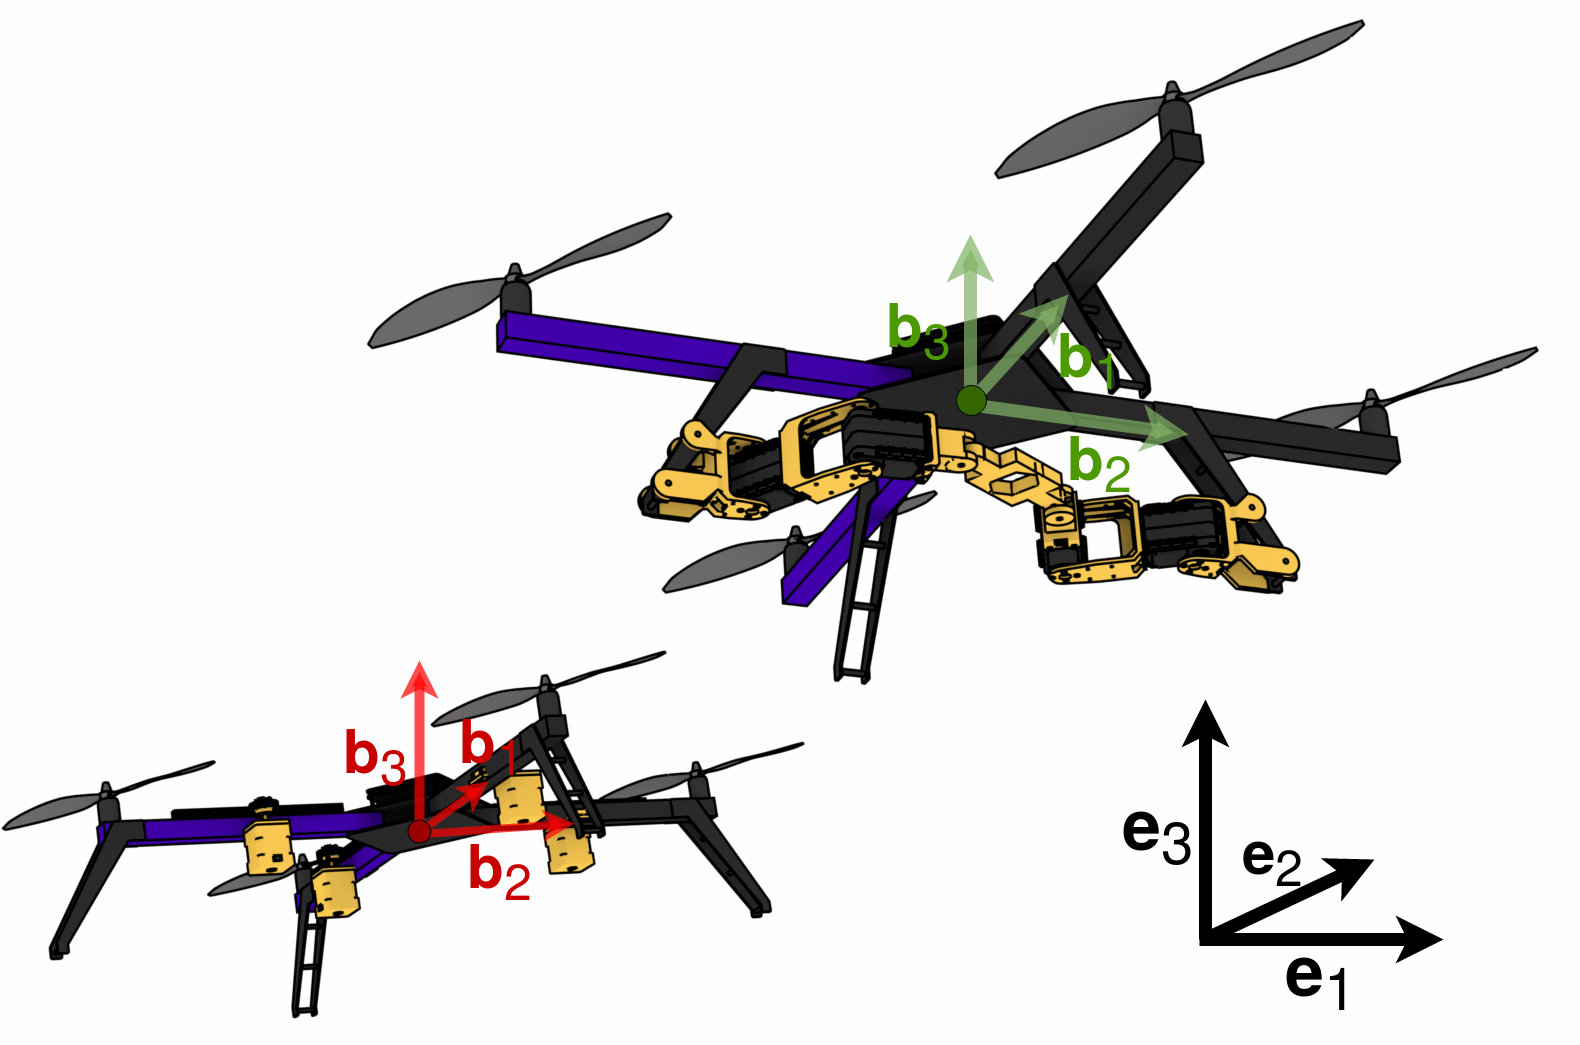
\includegraphics[width=0.85\columnwidth]{figure/uav.png}	
	\centering
	\caption{The $\text{figure}^{\cite{Markovic2019}}$ shows two UAVs endowed with variable moving masses (left) and manipulator carried payload (right). Both UAV concepts are able to offset their center of gravity outside the origin of their body-fixed frame $\{\textbf{b}_1, \textbf{b}_2, \textbf{b}_3\}$. The inertial frame is depicted as $\{\textbf{e}_1, \textbf{e}_2, \textbf{e}_3\}$.  }
	\label{fig:uav_model}
\end{figure}

Another widespread application of the geometric controller are payload transportation tasks. Originally introduced by T. Lee and V. Kumar 2013. \cite{cable-load1}, variations of the concept with multiple quadrotors carrying a payload was presented in \cite{cable-load-multiple} and \cite{Lee2014GeometricCO}. Quadrotor with a flexible cable model and attached load was presented in \cite{tethered-quadrotor}, \cite{flexible-cable}, \cite{flexible-cable-dynamics} and \cite{stabilization-flexible-cable}. Adaptive control along with unknown mass variations are presented in  \cite{rigid-body-transport} and \cite{unknown-mass-transport} respectively.
The overarching idea between all the mention papers considers an underactuated coordinate-free dynamic model of a quadrotor with a cable-suspended load defined on the configuration manifold SE(3)$\times\text{S}^2$, where $\text{S}^2 = \{\textbf{x} \in \mathbb{R}^{3} \,:\, \lVert \textbf{x} \rVert = r \}$. Coordinate-free approach is once again utilized to avoid singularities and complexities that are associated with local parameterizations. A nonlinear geometric control design is developed, that enables tracking of outputs defined by quadrotor and load attitude as well as position of the load. 

\begin{figure}[H]
	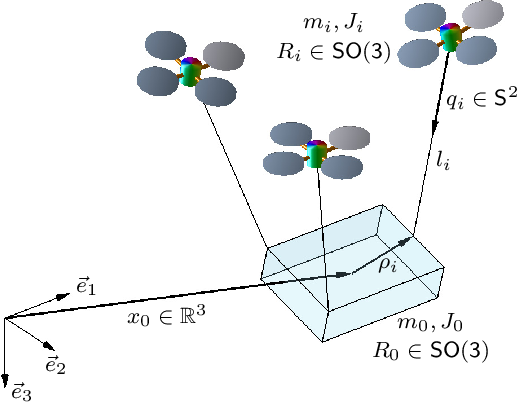
\includegraphics[width=\columnwidth]{figure/payload_carrying.png}	
	\centering
	\caption{This $\text{figure}^{\cite{Lee2014GeometricCO}}$ represents multiple quadrotor UAVs carrying a single rigid-body load via cables. Cable are defined in $\text{S}^2$ - spherical configuration while the UAV remains in SE(3). The underlying coupled system mechanics, therefore, evolve on an SE(3)$\times\text{S}^2$ configuration manifold. }
	\label{fig:load_carrying}
\end{figure}

\todo[inline]{Add Optimal Control...}

\section{Passivity-Based Control} \label{section:pssivity}
Initial presentation of passive-decomposition is found in D. Lee et. al 2004. \cite{passive-decomp-mechanical-coord-req}. It decomposes the overall dynamics into shape system addressing the coordination aspect, locked system representing internal dynamics wrt. the holonomic constraints and dynamic couplings between the locked and shape systems.The coupled dynamics can be canceled out without violating passivity. Thus, the coordination aspect (shape system) and the dynamics of the coordinated (locked) system can be decoupled from each other while enforcing passivity. By designing the locked and shape controls to enforce passivity  of their respective systems, the closed-loop system energetic passivity is guaranteed. A brief introduction towards passive-decomposition is given as follows. \\
Consider a group of $m$-mechanical systems such that the $i$-th agent's dynamics evolve on a configuration manifold $\Ma_i$:
	\begin{equation}
	M_i(\textbf{q}_i)\nabla^i_{\textbf{v}_i} \textbf{v}_i = \textbf{T}_i + \textbf{F}_i, \;\;\; i = 1,...,m,
\end{equation}
where the following terms are defined as follows:
\begin{itemize}
	\item $\textbf{T}_i, \textbf{F}_i\in\text{T}_{\textbf{q}_i}^*\Ma_i$ - control and environmental force covectors that exist in a cotangent manifold at point $\textbf{q}_i$
	
	\item $\textbf{v}_i \in \text{T}_i^{*}\Ma_i$ - system velocity at point $\textbf{q}_i$ in the tangent manifold
	
	\item $\nabla^i_{\textbf{v}_i}$ - this symbol represents a covariant derivative operator, the Levi-Civita connection. It provides a well defined method of differentiating vector fields along the ${\textbf{v}_i}$ direction on the tangent bundle $\text{T}\Ma_i$.
	
	\item $M_i(\textbf{q}_i)$ - inertia tensor which maps vectors from tangent space to cotangent space at point $\textbf{q}$, defined as $M:\text{T}_{\textbf{q}}\Ma \mapsto \text{T}_{\textbf{q}}^*\Ma$
\end{itemize}

Furthermore, the supply rate for the m-agent mechanical system is defined as follows.
\begin{equation}
	s_\rho(\textbf{v}_i, \textbf{T}_i) = \langle\textbf{F}_i, \dot{\textbf{q}}_i \rangle + ... + \langle\textbf{F}_m, \dot{\textbf{q}}_m \rangle \, ,
\end{equation}
where $\langle \cdot, \cdot \rangle: \text{T}_{\textbf{q}}^*\Ma \times \text{T}_{\textbf{q}}\Ma  \rightarrow \mathbb{R}$. \\
\noindent For safe and stable interaction an energetic passivity condition where $\exists d\in\mathbb{R}$ such that: 
\begin{equation}
	 \int_{0}^{t}	s_\rho(\textbf{v}_i(\tau), \textbf{T}_i(\tau))d\tau \geq -d^2, \;\forall t\geq 0
\end{equation}
Similar condition is employed to induce controller passivity. \\
Introducing the coordination map $h:\Ma^n \rightarrow \Na^m$ which holds the holonomic constraints, at each point of the configuration manifold $q\in\Ma$, the corresponding tangent space $\text{T}_q\Ma$
is split into two orthogonal vector spaces as follows:
\begin{equation}
	\text{T}_q\Ma = \text{T}_q^\top \Ma \oplus \text{T}_q^{\perp} \Ma
\end{equation}
The tangential and perpendicular spaces are defined respectively:
\begin{gather}
	\text{T}_q^\top\Ma := span \{v \in \text{T}_q\Ma \, \vert \, h_*(v) = 0\}  \\
	\text{T}_q^\perp\Ma := span \{w \in \text{T}_q\Ma \, \vert \, \langle \langle v, w \rangle \rangle, \, \forall v \in \text{T}_q^\top \Ma  \}, 
\end{gather}
where $h_*: \text{T}_q\Ma \rightarrow \text{T}_{h(q)}\Na$ is the push-forward of the coordination map. \\
By applying the orthogonal decomposition to the model dynamics we are able to decouple the shape and locked dynamics, while applying a control law cancel the coupling which essentially sums up the notion of passive-decomposition.

A concrete application of the passive-decomposition concepts on a UAV system can be found in \cite{passive-decomp-quadrotor-with-robotic-manip}. The authors show that the Lagrange dynamics of quadrotor-manipulator systems can be completely decoupled into: the center-of-mass dynamics in E(3), which, similar to the standard quadrotor dynamics, is point-mass dynamics with under-actuation  and  gravity  effect; the  “internal rotational” dynamics  of  the  quadrotor’s  rotation  and  manipulator configuration, which assumes the form of standard Lagrange dynamics  of  robotic manipulator with full-actuation and nogravity effect.  
\begin{figure}[H]
	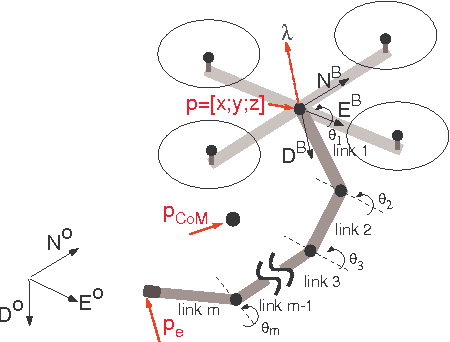
\includegraphics[width=0.95\columnwidth]{figure/aerial_manip.png}	
	\centering
	\caption{This $\text{figure}^{\cite{passive-decomp-quadrotor-with-robotic-manip}}$ represents a quadrotor UAV with a generalized m-DOF robot arm. The UAV platform's position is denoted with $\textbf{p}$, $\textbf{p}_e$ represents the end-effector position while $\textbf{p}_{CoM}$ is the center-of-mass vector of the entire quadrotor-manipulator system. It is worth nothing that a general case is considered where $\textbf{p}_{CoM} \neq\textbf{p}$.  }
	\label{fig:aerial_manip}
\end{figure}
\noindent A backstepping-like end-effector tracking control law is proposed, which allows  assignment of different roles for the center-of-mass control and internal rotational dynamics  control according to task objectives.

A similar passivity-based control design is presented in \cite{decoupled-aerial-manipulation} for quadrotor-manipulator UAV system utilizing a PID cascade  unlike the previously shown backstepping controller. Proposed control algorithms are implemented in the MATLAB/
Simulink environment and tested using the highly nonlinear system model in simulation. 
The controller robustness is checked by applying disturbance forces from different 
directions at the tip point of the 2-DOF robotic arm.

In \cite{passivity-backstepping}  a novel unified passivity-based adaptive backstepping control framework is proposed for ‘mixed’ quadrotor UAVs. Which consists of the translation dynamics with thrust force input and the attitude kinematics with the angular velocity input evolving on SE(3). Its application to haptic teleoperation over the Internet is also presented with dynamic-extension like filter to address discontinuous communication and a complete stability/collision-avoidance analysis is provided.

\cite{passivity-based-formation-load}
\cite{passive-variable-impedance-compliant} 
\cite{max-wrench-min-energy} 
\cite{quadrotor-itneraction-environment} 
\cite{passivity-based-payload-minimum-swing} 
\cite{passivity-based-crop} 
\cite{payload-and-human}
\cite{door-opening}
\cite{passivity-based-physical-interaction}
\section{Future Work} \label{future_work}
\section{Conclusion} \label{section:conclusion}
In this paper a survey on manifold-based UAV control methods is given. The focus is on geometric mechanics as well as the passive-decomposition framework. Both operate on the underlying SE(3) quadrotor configuration with appropriate modifications when endowed with n-DoF manipulators or cables carrying a payload. \\
The original geometric control concept is generally applied for trajectory tracking purposes for various configuration parts, i.e. UAV or payload center of mass. Other applications include time optimal trajectory or attitude tracking on the given configuration manifold. \\
Passive-decomposition opens a multitude of utilization opportunities by introducing a generalized rigid body control framework while enforcing energetic-passivity of the closed-loop system. Passivity-based control methods are applied in various research projects such as trajectory tracking of a quadrotor-manipulator system, physical environment interaction, achieving compliant behavior of UAVs, formation control, inspection etc. \\
Current state-of-the-art methods are presented for both of the mentioned control frameworks.

%%%%%%%%%%%%%%%%%%%%%%%%%%%%%%%%%%%%%%%%%%%%%%%%%%%%%%%%%%%%%%%%%%%%%%%%%%%%%%%%
%\section*{APPENDIX} \label{sec:appendix}
%\input{content/appendix.tex}

%Appendixes should appear before the acknowledgment.

\section*{ACKNOWLEDGMENT}

This research was supported by European Commission Horizon 2020 Programme through project under G. A. number 810321, named Twinning coordination action for spreading excellence in Aerial Robotics - AeRoTwin \cite{AEROTWINweb} and through project under G. A. number 820434, named ENergy aware BIM Cloud Platform in a COst-effective Building REnovation Context - ENCORE \cite{ENCOREweb}.
%%%%%%%%%%%%%%%%%%%%%%%%%%%%%%%%%%%%%%%%%%%%%%%%%%%%%%%%%%%%%%%%%%%%%%%%%%%%%%%%

%\nocite{*}
\bibliographystyle{ieeetr}
\bibliography{bibliography/Mendeley}
\end{document}
